\chapter{Iteration 8}
\label{it:8}
\section{Planning}
This main goal for this final iteration was to complete the post-processor and front-end web application. Finishing the detection methods implementations and displaying the metrics and chart in the staff dashboard. Below is the list of stories and their assigned story points. The list is displayed in completion order.

\begin{itemize}
\item Add post-processor tests: 3 points
\item Add full documentation to each module: 2 points
\item Add installation instructions: 2 points
\item Add submission graph visuals for staff dashboard: 3 points
\item Implement a plagiarism / UAC scale: 1 point
\end{itemize}

\section{Implementation}
\subsection{Testing the Post-Processor}
Due to the post-processor data structure not being well developed before implementation, unit tests were not appropriate at the time. Now that the data structure is mostly complete, it is now reasonable to add these unit tests. Currently, due to time restrictions, only one unit test was implemented. A simple input-process-output test. This test uses sample encrypted XML data, runs it through the post-processor, and a result is returned. The result is compared to the expected data.

\subsection{Documenting the Code}
Over the course of the last few sprints, code documentation has become scarce. A story was put into this sprint to accommodate for the lack of documentation, including installation instructions. Each module was fully documented with appropriate Javadocs, docstrings, and line comments where necessary. The installation instructions were added to the \texttt{README.md} file. These instructions also included system requirements. Separate instructions are documented for each module.

\subsection{Plotting Charts using Pygal}
Currently, Matplotlib was used for displaying the frequency vs. time chart. This only worked locally, but was useful for testing the chart data. Pygal will be used to display charts in the Flask application\cite{PygalFlask}. Matplotlib and Pygal share a very similar method of building charts. This made a smooth transition to Pygal to display the FTS (Frequency Time Source) data. Matplotlib will still used for local testing of charts.

The Pygal submission charts were added to the staff dashboard. Initially they were embedded directly into the table. This took up a lot of space and was aesthetically unpleasant. It was decided to add a new page which would display all submission details. This would keep the submissions table simple, providing a link to each submission detail page. The submission detail page uses this url format, \texttt{/dashboard/submission/<user\_uid>/<submission\_id>}. The staff dashboard table now has a link to access the submission details view (see \autoref{fig:web-all-submissions} in \autoref{sec:the-plagiarism-value-metric}).

The submission details page displays the metrics, FTS chart, and a list of \textit{large changes}. The metrics are displayed in a description list as shown below in \autoref{fig:web-submission-data}. The FTS chart is displayed as an SVG+XML image as shown below in \autoref{fig:web-submission-fts-chart}. This allowed the Pygal chart to provide interactivity. This interactivity includes selecting specific sources and tool tips showing discrete values. The large changes are displayed in a table as shown below in \autoref{fig:web-submission-changes}. A \textit{large change} is a change which meets a specific size requirement. The default size considered for a change to be \textit{large} is 200 characters. This can be configured by specifying a GET parameter in the URL. For example, \url{/dashboard/submission/abc12/5aca40cca326f6001046e1b8?large\_change\_size=91}. This url will show a specific submission where large changes are classed as having a size of 91 or greater. The total time metric for submissions was added which lead to the creation of the CPM (characters per minute) metric. The CPM is calculated by simply dividing the total frequency by the total time. The average CPM is between 190 and 200\cite{LiveChatTypingSpeedTest}. For professional typists the average CPM is between 325 and 375. However, the CPM when using IntelliJ could be drastically higher. Due to tracking every single change, auto-completion, automatic code generation, and refactoring all count towards the CPM. This will have to be taken into account when evaluating a submission. See \autoref{chp:results} for an in-depth review about the submission results.

\begin{figure}[H]
  \centering
  \fbox{
    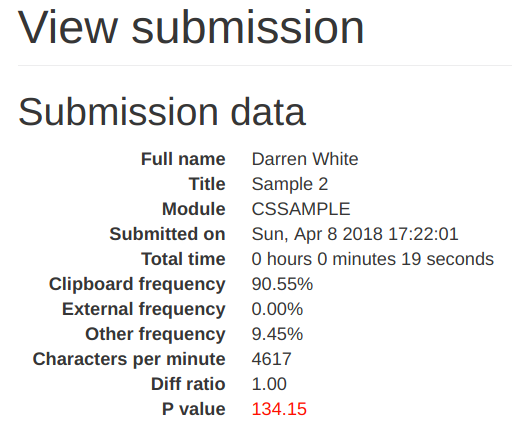
\includegraphics[height=.5\textheight,
    keepaspectratio=true,
    width=.5\textwidth,
    ]{figures/11-web-view-bad-submission-data.png}
  }
  \caption[Web Submission Data]{An example submission metrics view. This shows the submissions post-processed results.}
  \label{fig:web-submission-data}
\end{figure}

\begin{figure}[H]
  \centering
  \fbox{
    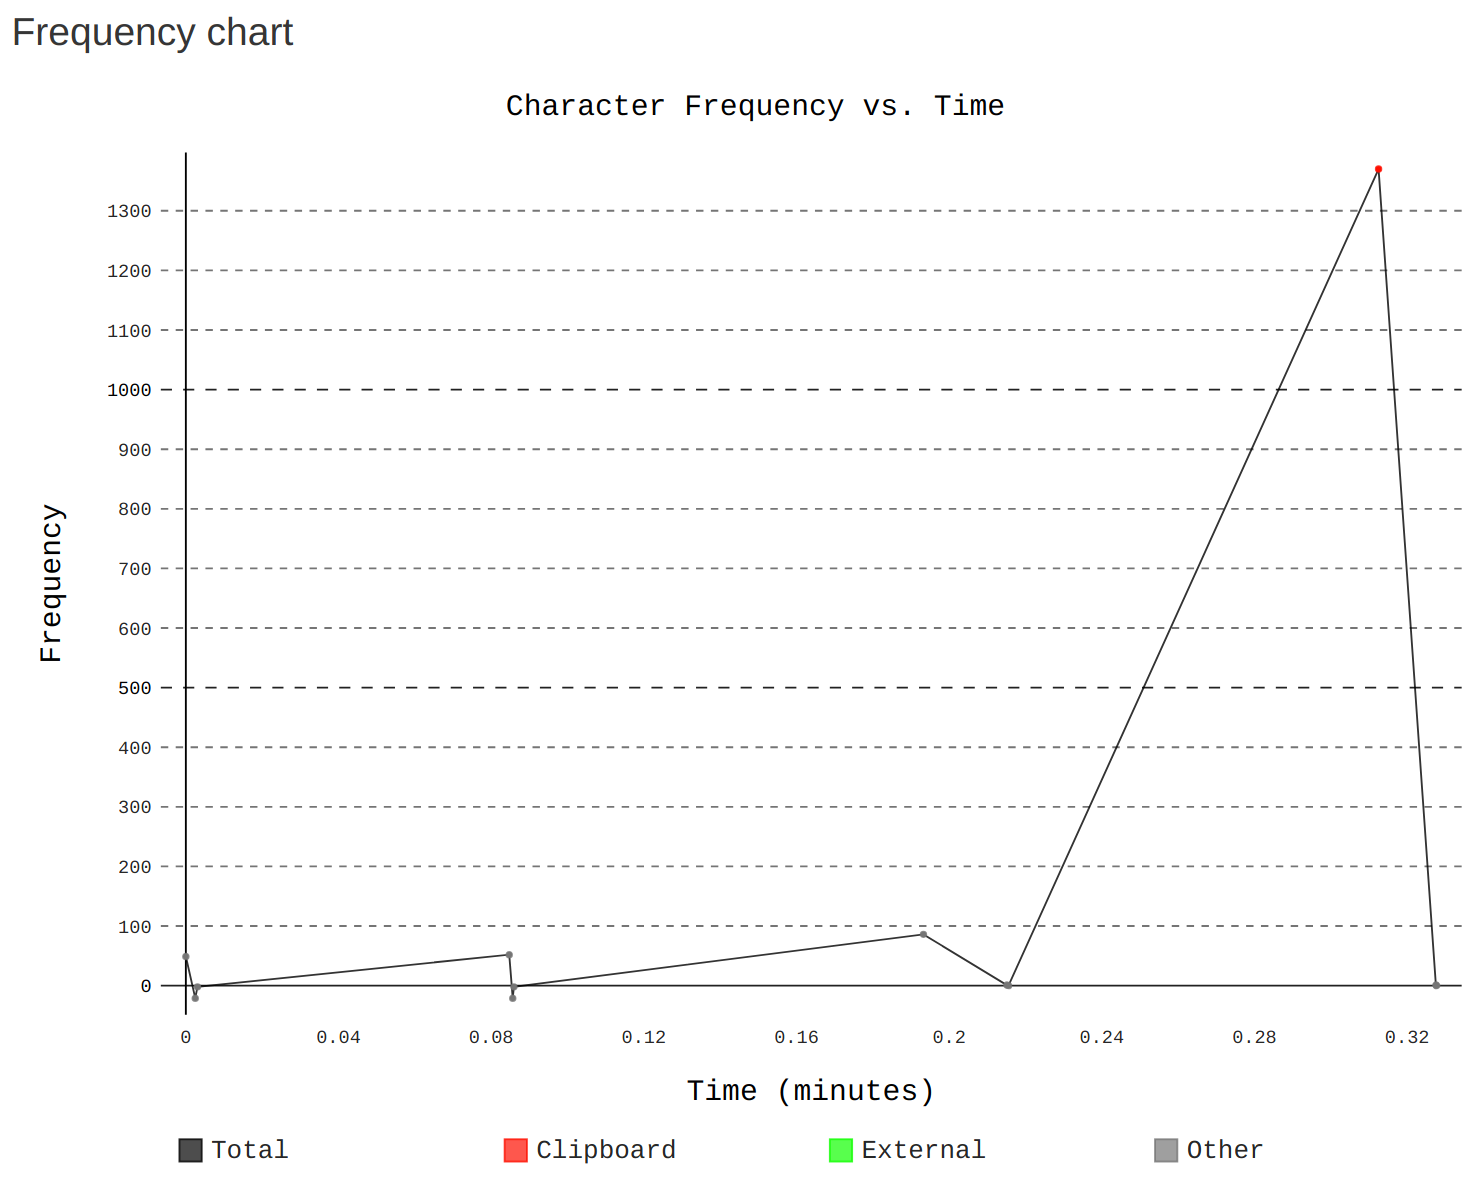
\includegraphics[height=.9\textheight,
    keepaspectratio=true,
    width=.9\textwidth,
    ]{figures/12-web-view-bad-submission-chart.png}
  }
  \caption[Web Submission FTS Chart]{An example submission FTS chart. This shows the type of source code changes over the development time of a submission.}
  \label{fig:web-submission-fts-chart}
\end{figure}

\begin{figure}[H]
  \centering
  \fbox{
    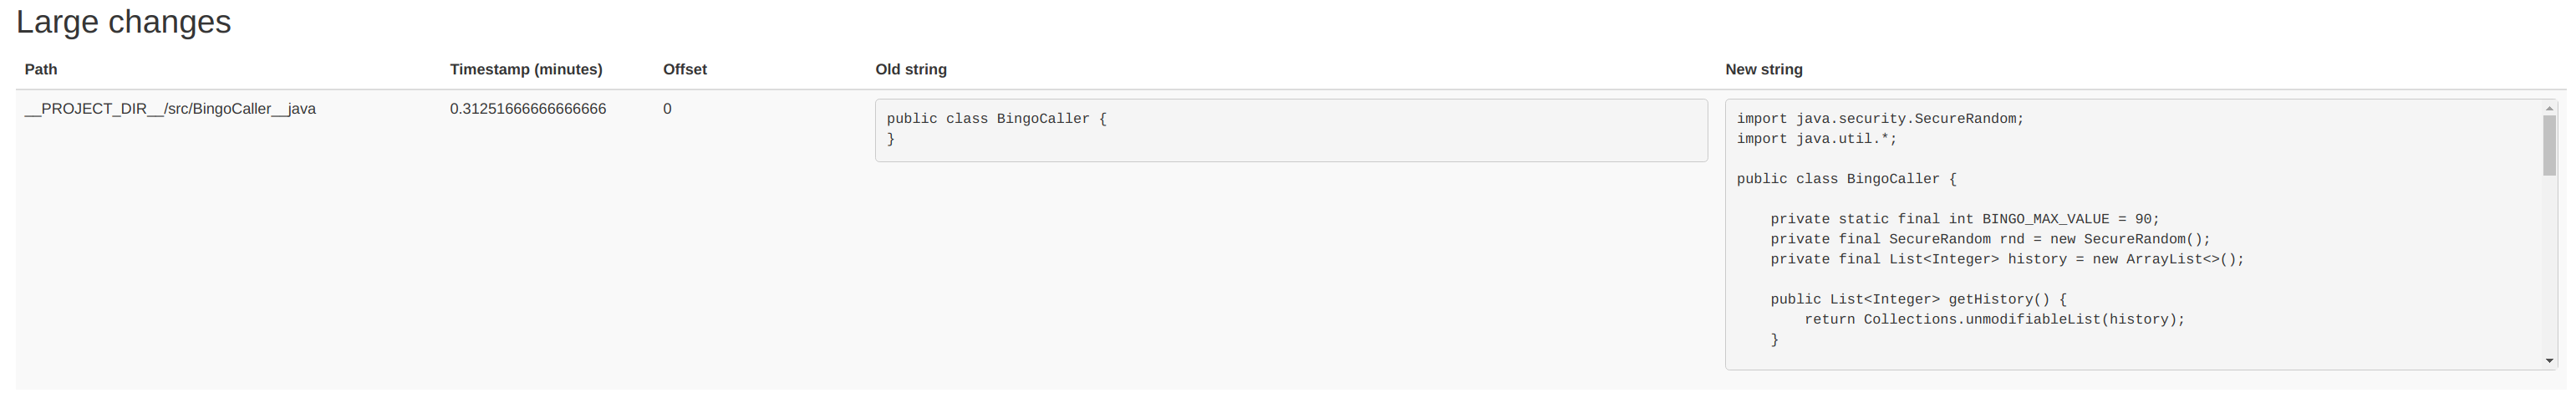
\includegraphics[height=\textheight,
    keepaspectratio=true,
    width=\textwidth,
    ]{figures/13-web-view-bad-submission-changes.png}
  }
  \caption[Web Submission Changes]{An example submission large changes. This shows the major changes tracked for a submission.}
  \label{fig:web-submission-changes}
\end{figure}

\subsection{The Plagiarism Value Metric}
\label{sec:the-plagiarism-value-metric}
The final metric to be added was the p\_value metric (i.e. the plagiarism value). This was calculated using all the metrics available. It also has an associated colour (low value is green, high value is red). The p\_value operates on a linear scale. Currently this scale is 0 to 40. This scale is only a guideline and may change in the future with more testing. A large range of samples would be required for a more accurate scale. The p\_value equation is shown below.

\[
  p\_value = \frac{t}{100} \cdot d \cdot ((c + 1) + (e + 1)^2)
\]

\begin{align*}
  \text{where}~t &= \text{Total time,} \\
  d &= \text{Diff ratio,} \\
  c &= \text{Clipboard change frequency,} \\
  e &= \text{External file change frequency}
\end{align*}

The clipboard and external change frequencies are added together. The external frequency is exponential because externally changing a file allows any kind of changes. The diff ratio acts as an accuracy modifier. Usually the diff ratio will be 1.0 so it will not affect the final value. The diff ratio will be less than 1.0 when one or more changes are not tracked. The longer the project was developed for, the smaller the p\_value. This means that projects developed extremely quickly will be flagged. The p\_value also has a colour associated with it. Depending on the value, the colour will gradually change. \autoref{cde:p-value-colour} shows the algorithm below for determining the colour for a p\_value. The \texttt{\_\_P\_VALUE\_LIMIT} is defined as 40. But this may change in the future.

%TC:ignore
\begin{code}
\begin{minted}[breaklines,
               linenos,
               frame=lines]{python}
mod = 255 / __P_VALUE_LIMIT
r = min(255, round(p_value * mod))
g = max(0, 255 - round(p_value * mod))
b = 0
\end{minted}
\caption{Python algorithm to calculate colour based on the p\_value}
\label{cde:p-value-colour}
\end{code}
%TC:endignore

\begin{figure}[H]
  \centering
  \fbox{
    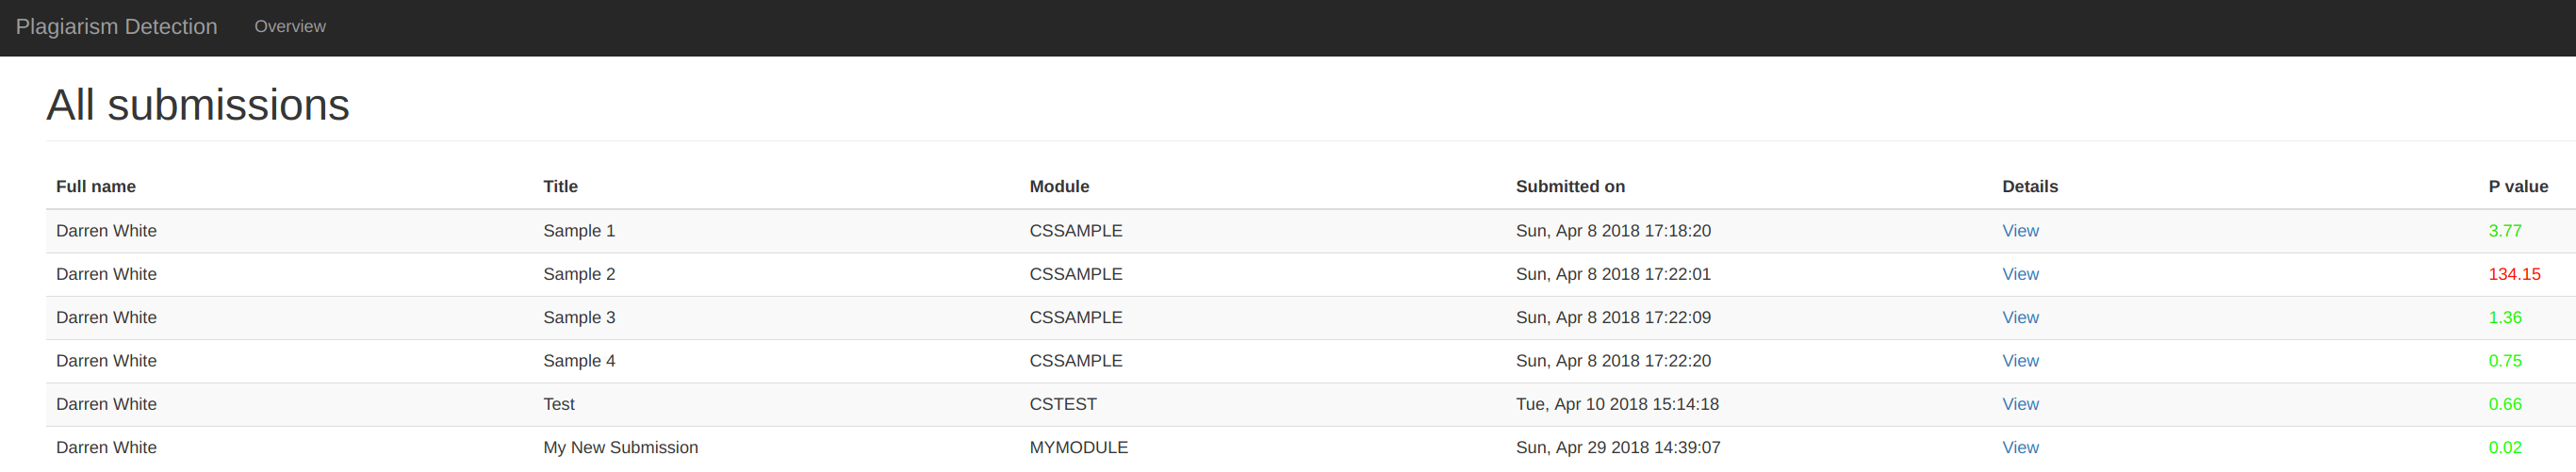
\includegraphics[height=\textheight,
    keepaspectratio=true,
    width=\textwidth,
    ]{figures/10-web-all-submissions.png}
  }
  \caption[Web Staff Dashboard All Submissions]{The staff dashboard with a view of all student submissions. The p\_value is shown in the far right column with its associated colour. The staff dashboard now has a link to view the submission details.}
  \label{fig:web-all-submissions}
\end{figure}

\section{Retrospective}
The velocity for this final iteration is 11. All of the development was completed during this iteration. The post-processor and front-end web application are now finished. The following chapters in this report will include the design architecture, testing, results analysis, evaluation, and conclusions.
